\documentclass[10pt,a4paper]{article}

\usepackage[margin=2.0cm]{geometry}
\usepackage[T1]{fontenc}
\usepackage{lmodern}
\usepackage{microtype}
\usepackage{amsmath,amssymb,bm}
\usepackage{graphicx}
\usepackage{booktabs}
\usepackage{multirow}
\usepackage{tabularx}
\usepackage{array}
\usepackage{xcolor}
\usepackage{enumitem}
\usepackage{caption}
\usepackage{subcaption}
\usepackage{float}
\usepackage[section]{placeins}
\usepackage{tikz}
\usetikzlibrary{arrows.meta,positioning,fit,backgrounds}
\usepackage{algorithm}
\usepackage{algpseudocode}
\usepackage[colorlinks=true,linkcolor=blue!50!black,citecolor=blue!50!black,urlcolor=blue!50!black]{hyperref}

\captionsetup{font=small,labelfont=bf}
\setlist{nosep,leftmargin=1.4em}
\newcommand{\pogs}{\textsc{Pogs}}
\newcommand{\kf}{KF}
\newcommand{\best}[1]{\textbf{#1}}
\newcolumntype{R}{>{\raggedleft\arraybackslash}X}

\title{\textbf{Re-implementing and Stress-Testing POGS}\\[0.3em]
\large A limitation-driven synthetic benchmark, an SE(3) Kalman motion prior,\\
and a real-time evaluation of Gaussian-splat object tracking}
\author{Md Nayeem}
\date{November 2026}

\begin{document}
\maketitle

\begin{abstract}
Persistent Object Gaussian Splat (\pogs{}) tracks scanned objects by optimising
their 6-DoF pose so that a Gaussian splat, rendered into the camera, matches
the observed DINO features and stereo depth. The paper reports results on a
physical robot at roughly 5\,Hz and names its own limitations: objects must
move slowly, and occlusion by hands or the gripper degrades tracking. This
report describes (i) an audited re-implementation of the \pogs{} pipeline that
follows the paper and the authors' release (scan, train, group, track);
(ii) a synthetic pick-and-place benchmark built around those limitations:
12 rendered conditions $\times$ 3 random trajectories, plus speed and depth-noise
settings, giving 54 cases with exact ground truth; (iii) a constant-velocity
SE(3) Kalman filter used as a warm start for the pose optimiser, with an
optional loss check; and (iv) a real-time protocol in which a 30\,Hz camera
stream is tracked with the tracker's \emph{measured} latency, so that a slow
tracker skips frames and publishes stale poses. Offline, the Kalman variant
with the loss check is the most accurate method overall (75\% vs.\ 71\%
ADD-S success, 16\% vs.\ 22\% lost frames). It holds 100\% at twice the object
speed, where \pogs{} falls to 82\%, and it fixes the cereal-box failure
(86\% vs.\ 57\%). In real time, \pogs{} with its published 25 iterations runs at
1.9\,Hz and is right on only 56\% of camera frames. Cutting it to 10 iterations,
or adding Kalman latency compensation, restores 100\% at normal speed. No method
survives a hand occluding the object, or the real-time stream played at twice
the speed.
\end{abstract}

\tableofcontents
\newpage

%==========================================================================
\section{Introduction}
%==========================================================================

\pogs{}~\cite{pogs} represents a scanned scene as 3D Gaussians~\cite{kerbl3dgs}
that carry, in addition to colour, a distilled DINO feature~\cite{dinov2} and a
hash-grid field of CLIP~\cite{clip} and instance-grouping features (in the style
of LERF~\cite{lerf} and GARField~\cite{garfield}). After grouping the Gaussians
into objects, each object's pose is tracked by gradient descent: the object's
Gaussians are rendered under a candidate rigid transform and compared with the
current camera frame's DINO features and stereo depth. The approach needs no
CAD model and no re-scan, and the paper uses it for object reset and tool
servoing on a physical robot.

The paper is candid about where this breaks: tracking runs at about 5\,Hz,
``objects had to be moved slowly'', and occlusion (by the gripper or a hand)
is a stated failure mode (Sec.~VI of~\cite{pogs}). Physical experiments make
these limits hard to quantify: there is no exact ground truth, and a condition
cannot be varied while holding everything else fixed. This project therefore
builds a controlled synthetic setting in which each limitation is a separate
\emph{factor} with several levels, re-implements \pogs{} faithfully, and tests
a modification against it on exactly the same cases.

\paragraph{Contributions.}
\begin{enumerate}
  \item \textbf{v1: an audited \pogs{} re-implementation} (Sec.~\ref{sec:v1}).
        Every default follows the paper or the release, and the source is cited
        in the code. Known deviations are listed explicitly (Table~\ref{tab:deviations}).
  \item \textbf{A limitation-driven benchmark} (Sec.~\ref{sec:dataset}): one
        scanned floor scene with five household objects, and a robot gripper that picks,
        carries and places a target under controlled rotation, speed,
        occlusion, depth-noise, object and multi-object conditions.
  \item \textbf{v2: an SE(3) Kalman motion prior} (Sec.~\ref{sec:v2}), plugged
        into the unchanged tracking loop as a warm start, with velocity damping,
        speed limits and an optional loss check. A compute sweep at 25/10/5
        optimiser iterations compares it with an equally cheap \pogs{}.
  \item \textbf{v3: other targets and two simultaneous objects}
        (Sec.~\ref{sec:v3}), drawn from the same run cache.
  \item \textbf{A real-time protocol} (Sec.~\ref{sec:realtime}): 30\,Hz renders of
        the same trajectories, a scheduler driven by measured latency, scoring
        at every camera frame, and Kalman latency compensation.
\end{enumerate}
Grasp planning, tool servoing and the physical robot are out of scope.

%==========================================================================
\section{Background: the POGS pipeline}
\label{sec:background}
%==========================================================================

Figure~\ref{fig:pipeline} summarises the four stages. We describe them as
implemented in v1; Section~\ref{sec:v1} lists the hyper-parameters.

\begin{figure}[t]
\centering
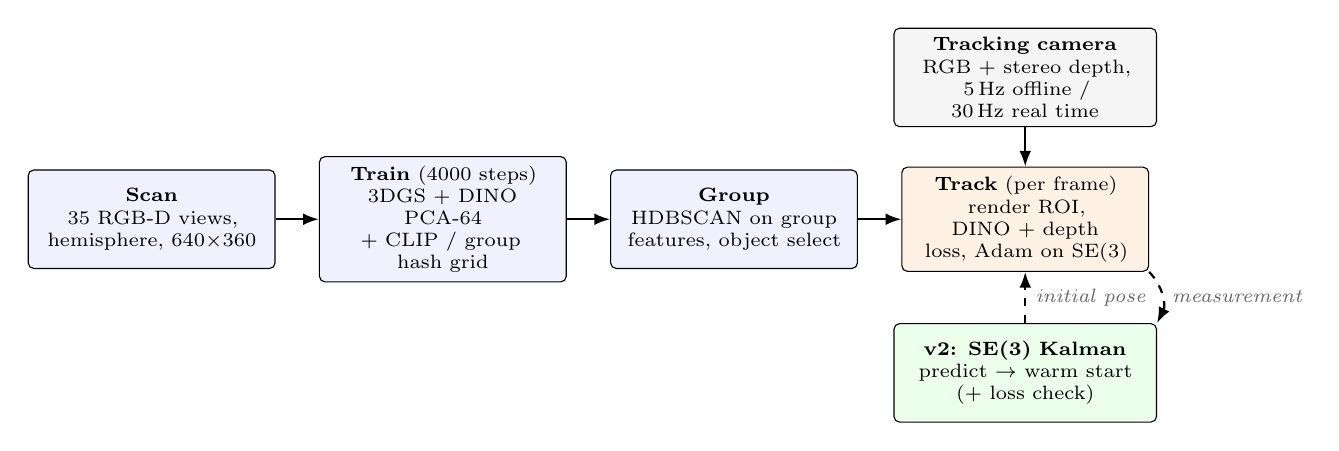
\begin{tikzpicture}[
  box/.style={draw, rounded corners=2pt, align=center, font=\scriptsize, minimum height=1.25cm, text width=2.9cm, fill=#1},
  box/.default=white,
  arr/.style={-{Latex[length=2mm]}, thick},
  lab/.style={font=\scriptsize\itshape, text=black!60}]
\node[box=blue!6] (scan) {\textbf{Scan}\\35 RGB-D views,\\hemisphere, 640$\times$360};
\node[box=blue!6, right=0.55cm of scan] (train) {\textbf{Train} (4000 steps)\\3DGS + DINO PCA-64\\+ CLIP / group hash grid};
\node[box=blue!6, right=0.55cm of train] (group) {\textbf{Group}\\HDBSCAN on group\\features, object select};
\node[box=orange!10, right=0.55cm of group] (track) {\textbf{Track} (per frame)\\render ROI, DINO + depth\\loss, Adam on SE(3)};
\draw[arr] (scan) -- (train);
\draw[arr] (train) -- (group);
\draw[arr] (group) -- (track);
\node[box=green!8, below=0.65cm of track, text width=3.1cm] (kf) {\textbf{v2: SE(3) Kalman}\\predict $\to$ warm start\\(+ loss check)};
\draw[arr, dashed] (kf) -- node[right, lab]{initial pose} (track);
\draw[arr, dashed] (track.south east) to[bend left=35] node[right, lab]{measurement} (kf.north east);
\node[box=gray!8, above=0.5cm of track, text width=3.1cm] (cam) {\textbf{Tracking camera}\\RGB + stereo depth,\\5\,Hz offline / 30\,Hz real time};
\draw[arr] (cam) -- (track);
\end{tikzpicture}
\caption{Pipeline. Blue: offline stages, run once per scene. Orange: per-frame
tracking (v1). Green: the v2 motion prior, which only changes the
optimiser's starting pose.}
\label{fig:pipeline}
\end{figure}

\paragraph{Training.} A splatfacto-style 3DGS model~\cite{nerfstudio,gsplat} is
fitted to the scan with an L1 + SSIM photometric loss and a Pearson depth loss.
Each Gaussian also carries a 64-D feature, supervised from step 100 to match
DINO ViT-S/14 features after a PCA from 384 to 64 dimensions. A 4-layer MLP
lifts the rendered feature back. From step 2500, a multi-scale hash grid is
supervised with CLIP embeddings (Huber loss) and with a contrastive
instance-grouping loss on detector masks. The masks are Detic-like~\cite{detic};
everything without a mask forms a ``negative'' mask. The PCA basis is part of
the checkpoint: tracking frames must be projected with the \emph{same} basis.

\paragraph{Grouping.} Gaussians are clustered on their grouping features with
HDBSCAN~\cite{hdbscan}. The release asks an operator to click the object to
track. We select clusters geometrically instead, after the release's
support-plane cut (Gaussians below table height + 1.5\,cm are dropped). Clusters
are rejected if they are a support surface (robust XY footprint), background
(cosine similarity to the negative-mask target), or a fragment.

\paragraph{Tracking.} The RigidGroupOptimizer~\cite{rsrd,pogs} keeps one rigid
transform per object, a translation of the centroid and a world-frame
rotation about it. At each frame it renders the object's Gaussians inside a
region of interest (ROI) around the last estimate and minimises
\begin{equation}
  \mathcal{L} \;=\; \frac{1}{|\Omega|}\sum_{u\in\Omega}\big\|\,\hat f(u) - f(u)\,\big\|_2
  \;+\; \lambda_d\,\frac{1}{|\mathcal{V}|}\sum_{u\in\mathcal{V}}\big(\hat d(u)-d(u)\big)^2\,
  \mathbb{1}\!\left[(\hat d - d)^2 < \tau_d^2\right],
  \label{eq:trackloss}
\end{equation}
where $\hat f, \hat d$ are the rendered DINO feature and depth, $f, d$ the
observed ones, $\lambda_d = 3.7$, and $\tau_d = 0.26$\,m. Residuals above
$\tau_d$ (occluders, background) are ignored. The optimiser runs Adam for
25 iterations per frame, with the learning rate decaying from 0.004 to 0.0008.
The pose is initialised once, with 100 DINO-only iterations on the full frame
followed by 70 iterations with depth and ROI.

%==========================================================================
\section{Synthetic dataset}
\label{sec:dataset}
%==========================================================================

All data come from an analytic ray-caster written for this project
(\texttt{scene\_generator/}). It renders RGB, metric depth and instance ids with
shadows and a Blinn--Phong-style specular term. Because the generator knows every
object's pose exactly, ground truth is exact. One scene and one trained model
serve every tracking condition, so differences between conditions come from the
condition alone.

\subsection{Scene}
\label{sec:scene}

The scene is a tiled floor with a low wooden staging table
($40\times32$\,cm, top at 6\,cm) and five household objects standing on the floor
around it (Table~\ref{tab:objects}). The robot carries the target from the floor
onto the table.

\begin{table}[h]
\centering\small
\caption{Scene objects (scene v2). Size is the axis-aligned extent. All objects
start on the floor; the table is the placement target.}
\label{tab:objects}
\begin{tabularx}{\linewidth}{l l X l l}
\toprule
Object & Size (cm) & Material (pattern, roughness) & Role & Target in \\
\midrule
ceramic mug    & $10.4\times7.6\times9.7$  & glossy glaze (noise, 0.12), cream inside, coffee & default target & all factors \\
mustard bottle & $7.2\times4.8\times16.3$  & plastic with a printed label band (stripes) & target & \emph{object} \\
soup can       & $6.6\times7.4\times9.9$   & two-tone label (split), brushed tin lids & 2nd mover & \emph{multi-object} \\
red apple      & $7.6\times7.6\times8.2$   & skin patches (blotch) & distractor & -- \\
cereal box     & $7.2\times11.3\times15.0$ & printed box art (blotch, blue/yellow) & target & \emph{object} \\
table / floor  & --                        & wood grain / tiles with grout & support, background & -- \\
\bottomrule
\end{tabularx}
\end{table}

\paragraph{Scene v2.} The first version of the generator (v1) evaluated
procedural textures in \emph{world} coordinates. A carried object therefore
slid underneath a fixed pattern, which corrupts exactly the appearance
features that \pogs{} tracks. Version 2 evaluates every material in the hit
primitive's own frame ($\mathbf{x}_{\text{loc}} = R^\top(\mathbf{x}-\mathbf{t})$),
so textures move rigidly with the objects. Noise uses an integer lattice hash,
so CPU and GPU renders are bit-identical. Version 2 also adds roughness and
metallic parameters to the specular term. It fixes the table top at its nominal
height (it was 6\,mm higher, so placed objects sank into it) and moves the mug
and soup can clear of the table footprint. A unit test checks that every
footprint is at least 2\,cm from the table and from every other object.
Datasets, checkpoints and cached runs carry a \texttt{scene\_version} and
are regenerated when it changes. All results in this report use scene v2.

\subsection{Scan (training data)}

The scan has 35 views on a hemisphere of radius 0.68\,m, at elevations
30--75$^\circ$ around the scene centre, rendered at $640\times360$ with a 62$^\circ$
field of view (Fig.~\ref{fig:scan}). Depth gets stereo-like noise of 3\,mm
standard deviation at 0.7\,m, growing linearly with range. The initial point
cloud is back-projected from the depth maps and balanced per object (at most
2500 seed points per object, 4000 for the floor, 2500 for the table). Instance
masks are filtered like Detic output: the floor and table are not reported,
and masks larger than $1/3.5$ of the image are dropped.

\begin{figure}[t]
\centering
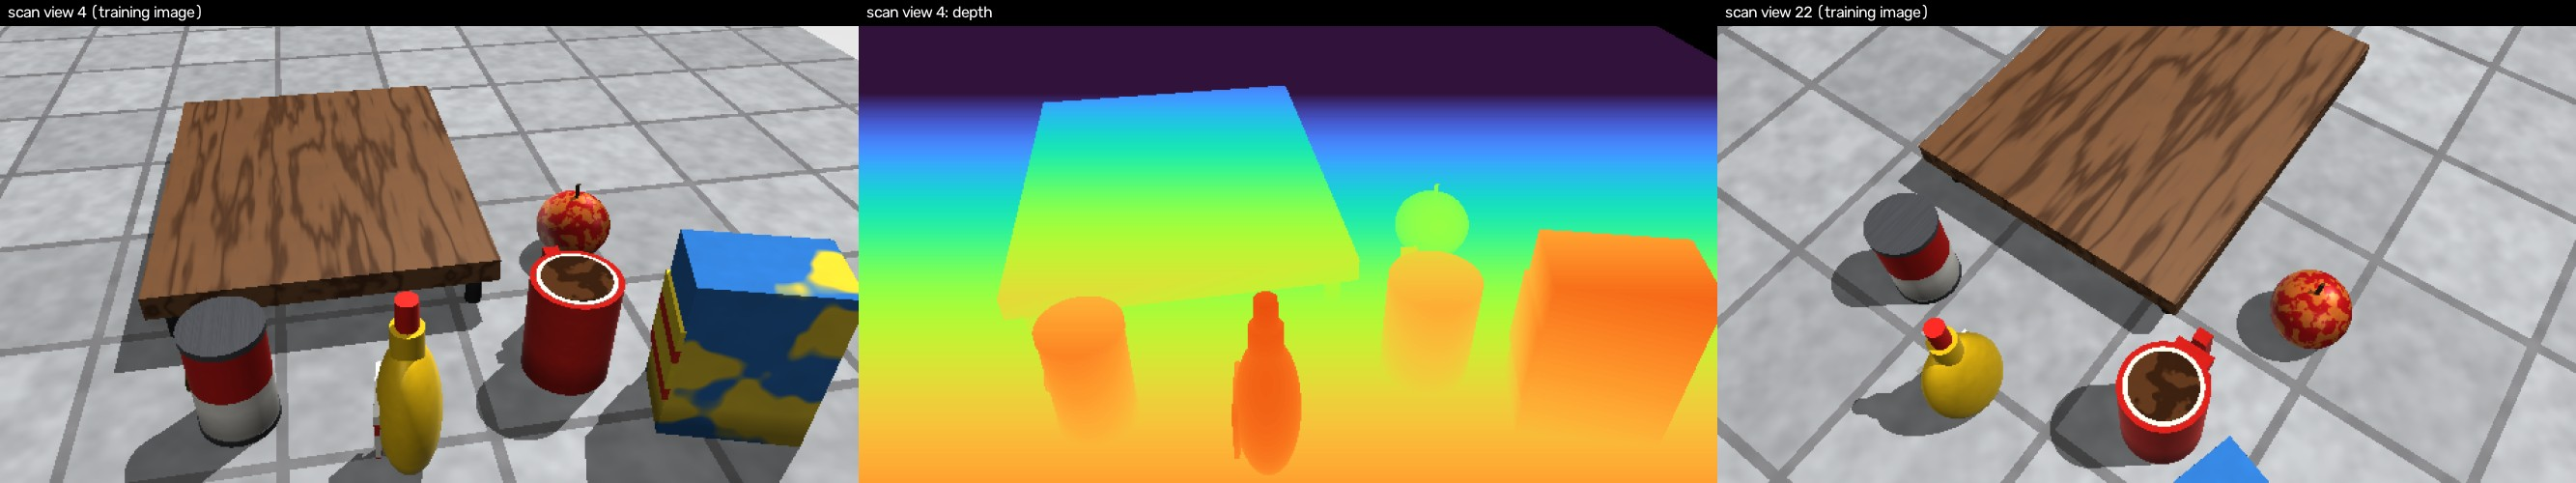
\includegraphics[width=\linewidth]{figures/scan_views.jpg}
\caption{Two scan views (left, right) and the depth map of the left view
(centre; near is warm). Materials: wood-grain table, tiled floor, glazed
mug, labelled bottle and can, printed cereal box, patchy apple skin.}
\label{fig:scan}
\end{figure}

\subsection{Tracking sequences}

A static tracking camera ($889\times500$, $f_x = 700$\,px, at
$(0.24, -0.70, 0.54)$\,m) watches a robot gripper (scaled to 0.7 of the stock
model) pick up the target, carry it and place it on the table. The base rate is
60 frames at 5\,Hz (12\,s), the rate the paper reports. Each trajectory has five
phases, defined as fractions of the object's active window:
\begin{center}\small
\begin{tabular}{llp{9.5cm}}
\toprule
0.00--0.12 & approach & gripper descends onto the object (object static) \\
0.12--0.25 & lift     & to carry height (9--12\,cm above the base, sampled) \\
0.25--0.75 & carry    & transit to the table with the condition's rotation profile \\
0.75--0.88 & place    & descend onto the table top (upright, final yaw) \\
0.88--1.00 & release  & gripper rises out of view (object static) \\
\bottomrule
\end{tabular}
\end{center}
With $s\in[0,1]$ the carry progress, the rotation profiles are:
\textit{yaw}, $\psi = \pm\,\theta s$; \textit{tilt},
$\phi = \theta\sin(\pi s)$ about a random horizontal axis, upright again at
placement; and \textit{combined}, both together with the tilt peak equal to the
total yaw. Each condition has three random trajectories (\emph{seeds}). They
vary the placement point on the table, the carry height, the path wobble, the
rotation sign and the tilt axis. Figure~\ref{fig:traj} plots the resulting
motion and occlusion profiles.

\begin{figure}[t]
\centering
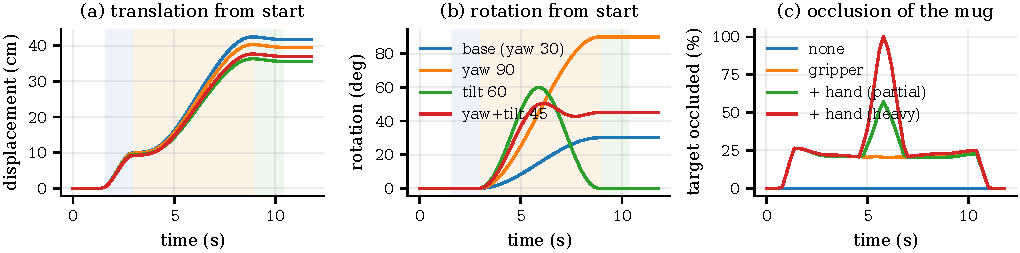
\includegraphics[width=\linewidth]{figures/trajectories.pdf}
\caption{Ground-truth profiles (seed 0). (a) Translation of the target from its
start; (b) total rotation angle; shading marks lift (blue), carry (orange) and
place (green). (c) Fraction of the mug's pixels hidden by the gripper and hand:
the gripper alone hides about 20\% while it holds the mug; the hand sweep peaks
at 57\% (partial) and 100\% (heavy).}
\label{fig:traj}
\end{figure}

\subsection{Conditions and factors}

The base condition is: mug target, net yaw of 30$^\circ$, gripper visible, 1$\times$
speed, 3\,mm stereo depth noise. Each factor changes one aspect of the base
condition (Table~\ref{tab:factors}; one frame per rendered condition in
Fig.~\ref{fig:conditions}). Speed and depth are applied at load time, without
re-rendering. \emph{Speed} $k$ keeps every $k$-th frame at the same camera rate, so
the object moves $k$ times further per tracked frame; equivalently, the tracker
is $k$ times slower than the camera. \emph{Depth} applies one of three noise
profiles deterministically. With three seeds per level, the six factors expand to
54 tracking cases. The base case appears in every factor as the reference level.

\begin{table}[t]
\centering\small
\caption{Benchmark factors. Each level differs from the base case
(\textbf{bold}) in one aspect only. Every level has three seeds.}
\label{tab:factors}
\begin{tabularx}{\linewidth}{l X X}
\toprule
Factor & Levels & Limitation probed (paper section) \\
\midrule
rotation     & yaw 15, \textbf{yaw 30}, yaw 90, tilt 30, tilt 60, yaw+tilt 45 & large rotations; tilt exposes the unscanned underside (Sec.~III assumptions) \\
speed        & \textbf{1$\times$}, 2$\times$, 4$\times$ on base and on yaw 90 & ``objects had to be moved slowly'' (Sec.~VI) \\
occlusion    & none, \textbf{gripper}, gripper + hand (partial, 57\% peak), gripper + hand (heavy, 100\% peak) & occlusion by gripper / human (Sec.~VI) \\
depth        & clean, \textbf{stereo 3\,mm}, noisy 10\,mm + 5\% holes & reliance on stereo depth \\
object       & \textbf{mug}, mustard bottle (thin, near-symmetric), cereal box (large, flat) & shape generality \\
multi-object & \textbf{one moving}, two moving (mug + soup can, two grippers) & simultaneous tracking \\
\bottomrule
\end{tabularx}
\end{table}

\begin{figure}[p]
\centering
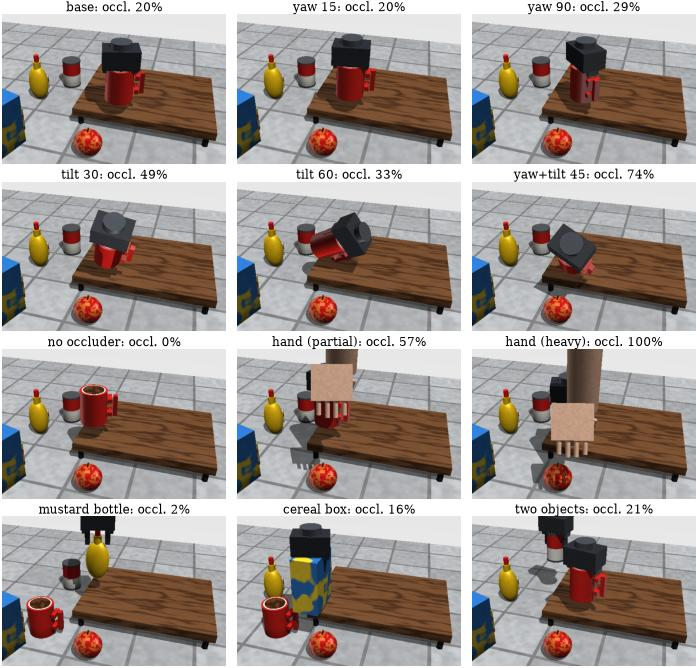
\includegraphics[width=\linewidth]{figures/conditions.jpg}
\caption{One tracking-camera frame per rendered condition (seed 0, cropped):
mid-carry for yaw conditions, peak tilt for tilt conditions, and peak occlusion
for hand conditions. Titles give the fraction of the target hidden in that frame.}
\label{fig:conditions}
\end{figure}

\subsection{Real-time sequences}

For the real-time protocol (Sec.~\ref{sec:realtime}), the base trajectories are
also rendered at 30\,Hz: 355 frames, where frame $6k$ of the 30\,Hz sequence is
frame $k$ of the 5\,Hz one. The motion is identical; only the camera samples it
six times more often. A playback speed of $k\times$ divides the timestamps by $k$
without re-rendering.

\subsection{Ground truth and storage}

Every frame stores RGB, depth in millimetres (\texttt{uint16}), instance masks,
the phase, the rotation angle, per-object occlusion fractions, and the
world-frame ground-truth motion of every object ($\mathbf{x}' = R\mathbf{x}+\mathbf{t}$,
the same transform the renderer applies). Ground truth is used only for
evaluation. It is never used to build groups, select objects or initialise
poses, and a code rule enforces this.

%==========================================================================
\section{Methods}
\label{sec:methods}
%==========================================================================

\subsection{v1: base POGS}
\label{sec:v1}

v1 follows the paper and the release. Table~\ref{tab:hparams} lists the settings
that matter most. Each value lives in \texttt{common/config.py}, whose docstrings
cite the release source.

\begin{table}[t]
\centering\small
\caption{Key v1 settings (all as in the paper or the release).}
\label{tab:hparams}
\begin{tabularx}{\linewidth}{l X}
\toprule
Stage & Setting \\
\midrule
Training & 4000 steps; DINO from step 100, CLIP + grouping from step 2500; splatfacto learning rates and densification (every 100 steps, gradient threshold 0.0008); SH degree 3; L1+SSIM ($\lambda = 0.2$) + 0.05$\times$Pearson depth; gradient accumulation 3 for the hash-grid field \\
DINO & ViT-S/14, long side 1260\,px, PCA 384$\to$64 stored in the checkpoint, 4-layer MLP \\
Grouping & HDBSCAN (min.\ cluster 300, min.\ samples 50), 3-NN feature smoothing; support cut at 1.5\,cm; support surface if 5--95\% XY footprint $>0.06$\,m$^2$; background if similarity to the negative target $>0.98$ \\
Tracking & DINO L2 + 3.7$\times$depth (ignore 0.26\,m); Adam, lr $0.004\to0.0008$, 25 iterations per frame; ROI inflation 25\% + 75\,px, ROI $\le$ 490\,px; match resolution 500\,px; only the selected objects are rendered \\
Initialisation & 100 DINO-only iterations on the full frame + 70 with depth and ROI; lr 0.005; from the scan pose \\
\bottomrule
\end{tabularx}
\end{table}

\paragraph{Variants.} The paper states that the tracking loss combines the
feature and depth terms, but the release's per-frame \texttt{step()} defaults to
\texttt{use\_depth=False} and uses depth only during initialisation. v1 therefore
reports both: \textbf{POGS} (paper, depth every frame) and \textbf{POGS (release)}
(depth only at initialisation). The paper's ablations \textbf{No Depth} and
\textbf{No DINO (RGB)} run on the base condition.

\paragraph{Protocol.} As in the paper (Sec.~IV-C), only the manipulated
object(s) are tracked: the operator clicks the object to follow. Tracking all
five objects drags the static ones whenever the gripper or the carried object
passes through their ROI (12\,cm drift in a smoke test).

\begin{table}[t]
\centering\small
\caption{Intentional, documented deviations from the release.}
\label{tab:deviations}
\begin{tabularx}{\linewidth}{l X}
\toprule
Deviation & Reason \\
\midrule
Geometric object selection & replaces the operator's click; same support-plane cut as the release \\
Simulated Detic masks & instance masks from the renderer, filtered like Detic (floor and table join the negative mask) \\
CPU HDBSCAN on a subsample & cuML not available; at most 25k points clustered, labels propagated \\
No camera-pose optimiser & synthetic camera poses are exact \\
Mask fallback & if the accumulation $>0.9$ mask is empty, fall back to half the peak instead of crashing (counted) \\
Faster group transform & compose the $K$ group transforms, then \texttt{index\_select}; same maths as the Warp kernel, about 8$\times$ faster \\
\bottomrule
\end{tabularx}
\end{table}

\subsection{v2: SE(3) Kalman motion prior}
\label{sec:v2}

\paragraph{Motivation.} \pogs{} starts each frame's optimisation from the previous
frame's estimate. When the object moves further between frames than 25 Adam steps
can cover, the estimate lags, the ROI drifts off the object, and tracking is lost.
A motion model can predict where the object will be and start the optimiser there.

\paragraph{State and dynamics.} One filter runs per tracked object. Its state is
expressed in exactly the parameters \pogs{} optimises: the centroid translation
$\mathbf{p}$ and the world-frame rotation $\mathbf{q}$, plus a linear velocity
$\mathbf{v}$ and an angular velocity $\bm{\omega}$. Translation and rotation are
two independent constant-velocity models driven by white-noise acceleration
(Bar-Shalom et al.~\cite{barshalom}). Rotation uses an error-state formulation:
the nominal quaternion is propagated as $\mathbf{q}\leftarrow\exp(\bm{\omega}\,\Delta t)\otimes\mathbf{q}$,
and the 3-D error lives in the tangent space, so there is no Euler singularity
and no yaw-only restriction. For a step $\Delta t$ and damping
$\alpha = e^{-\Delta t/\tau}$,
\begin{equation}
F = \begin{bmatrix} I_3 & \Delta t\,I_3 \\ 0 & \alpha\,I_3\end{bmatrix},\qquad
Q = \sigma_a^2 \begin{bmatrix} \tfrac{\Delta t^4}{4} I_3 & \tfrac{\Delta t^3}{2} I_3\\[2pt]
\tfrac{\Delta t^3}{2} I_3 & \Delta t^2 I_3\end{bmatrix},\qquad
H = \begin{bmatrix} I_3 & 0\end{bmatrix},
\end{equation}
with $\sigma_a = 0.5$\,m/s$^2$ for translation and $4$\,rad/s$^2$ for rotation. The
measurement is the optimiser's converged pose, with $\sigma_p = 1$\,cm and
$\sigma_\theta = 0.06$\,rad.

\paragraph{Stabilisation.} An undamped filter diverged by metres once tracking
slipped. The warm-started optimiser's output is not independent of the
prediction, so a wrong velocity re-confirms itself. v2 therefore damps velocity
with $\tau = 1$\,s (velocity decays unless measurements sustain it), clamps
speed at $|\mathbf{v}|\le0.5$\,m/s and $|\bm{\omega}|\le3$\,rad/s, and records the
normalised innovation squared (NIS) for consistency checks.

\paragraph{Variants.} \textbf{POGS + KF} starts every frame from the prediction.
\textbf{POGS + KF + check} renders the tracking loss at both the prediction and
the previous estimate before optimising, and keeps the prediction only where it
lowers the loss (greedy, per object). This guards against bad predictions. A
\emph{fuse} variant, which replaced the optimiser's output with the filtered
estimate, double-counted the prior and was dropped. A speed claim needs an
equally cheap baseline, so v2 also runs every method at 10 and 5 optimiser
iterations per frame, next to plain \pogs{} at the same budget.

\paragraph{Latency compensation.} The filter accepts a variable $\Delta t$, so it
can predict across the uneven gaps of the real-time protocol. It can also
extrapolate an estimate to ``now'' without changing its state. With damping,
the expected displacement over a horizon $\Delta$ is the damped velocity integral
\begin{equation}
\mathbf{p}(t+\Delta) = \mathbf{p}(t) + \mathbf{v}\,\tau\,(1-e^{-\Delta/\tau}),\qquad
\mathbf{q}(t+\Delta) = \exp\!\big(\bm{\omega}\,\tau(1-e^{-\Delta/\tau})\big)\otimes\mathbf{q}(t).
\label{eq:extrap}
\end{equation}
Methods marked \textbf{+ latency comp.} publish this extrapolated pose. The
optimisation itself is unchanged, so they share the run of the base method.

\subsection{v3: other targets and two moving objects}
\label{sec:v3}

v3 uses the same scene, checkpoint and grouping as v1 and v2. It reports the
\emph{object} factor (mug, mustard bottle, cereal box) and the
\emph{multi-object} factor (mug and soup can carried at the same time by two
grippers) for \pogs{}, \pogs{} (release) and \pogs{} + KF. All three share
the run cache, so cases that v1 or v2 already tracked are not repeated.

\subsection{Real-time protocol}
\label{sec:realtime}

The offline benchmark tracks \emph{every} frame and ignores compute time. A
deployed tracker sees a camera stream instead. While it works on one frame, new
frames arrive, and the pose it publishes describes the past. The real-time
protocol (Algorithm~\ref{alg:rt}) simulates this with the tracker's
\emph{measured} compute time on this machine.

\begin{algorithm}[t]
\caption{Real-time evaluation (\texttt{common.evaluate.track\_realtime})}
\label{alg:rt}
\begin{algorithmic}[1]
\Require camera timestamps $t_0..t_{N-1}$ (30\,Hz, divided by the playback speed), tracker, optional Kalman prior
\State initialise on frame 0 (untimed: the object is at rest); $t_{\text{free}} \gets 0$, $\ell \gets -1$
\While{true}
  \State $j \gets$ newest frame with $t_j \le t_{\text{free}}$ and $j>\ell$; if none, $j \gets \ell+1$ \Comment{skip stale frames}
  \If{$j \ge N$} \textbf{break} \EndIf
  \State $s \gets \max(t_{\text{free}}, t_j)$; predict the KF over $t_j - t_\ell$ (true gap)
  \State track frame $j$; measure compute time $c$ (GPU-synchronised)
  \State publish the estimate of frame $j$ at time $s + c$; $t_{\text{free}} \gets s+c$; $\ell \gets j$
\EndWhile
\State \textbf{score} every camera frame $i$ on the last estimate published at or before $t_i$
\State \phantom{\textbf{score}} (\textit{+ latency comp.}: that estimate extrapolated by Eq.~\eqref{eq:extrap} to $t_i$)
\end{algorithmic}
\end{algorithm}

Besides accuracy, the protocol reports the latency (compute per tracked frame),
the tracker rate, the number of frames skipped per tracked frame, and the
\emph{estimate age}: how old the camera frame behind the published pose is.
Timings depend on the GPU and on anything else running on it, so all real-time
runs were made with the GPU otherwise idle (one NVIDIA RTX 4070).

%==========================================================================
\section{Evaluation protocol}
\label{sec:eval}
%==========================================================================

\paragraph{Metrics.} Errors are computed against the exact ground truth of the
target object, at every frame.
\begin{itemize}
  \item \textbf{ADD-S success}: the fraction of frames whose ADD-S (the mean
        distance from each transformed model point to its closest ground-truth
        point, which is symmetry-aware~\cite{posecnn}) is below 10\% of the object
        diameter. This is the main metric.
  \item \textbf{Lost}: the fraction of frames with centroid position error above 10\,cm.
  \item \textbf{Median position error} (cm) and \textbf{mean rotation error} (deg).
  \item The paper's \textbf{3\,cm \& 5$^\circ$} rule. We report it but do not rank
        methods by it. Whenever the gripper is in view, it stays at 10--20\% for every
        tracker (about 35\% without an occluder), because the gripper tilts the
        held mug by $\sim$20$^\circ$ in the estimate (Sec.~\ref{sec:rot}).
\end{itemize}

\paragraph{Baselines and statistics.} Every table includes \textbf{Static (no
motion)}, which always predicts the scan pose. It is right while the object
rests ($\approx$20\% of frames) and wrong afterwards, so it is the floor that a
tracker must beat. Means are over three seeds, and $\pm$ is the sample standard
deviation across seeds. Methods are compared on identical cases only. A method
name is a key of a shared run cache (\texttt{data\_results/benchmark\_runs}), so
one name always means one configuration and no run is repeated across v1, v2 and v3.

%==========================================================================
\section{Results}
\label{sec:results}
%==========================================================================

\subsection{Reconstruction and grouping}

The model trains in 11.7\,min to 332k Gaussians, with a train-view PSNR of
34.1\,dB and a mean depth error of 0.63\,cm (Fig.~\ref{fig:training}). Scene v1
reached 31.3\,dB and 2.6\,cm. Grouping finds six HDBSCAN clusters. Selection
keeps the five objects and rejects the floor and table (Fig.~\ref{fig:grouping}),
with IoU against the true object Gaussians of 0.98 (mustard), 0.95 (apple),
0.88 (cereal), 0.80 (mug) and 0.67 (soup can). Cluster purity is 0.87, and there
are no missing or duplicate objects.

On scene v2, the release thresholds first rejected three objects. A few hundred
stray floor Gaussians in the mustard and soup clusters inflated their min/max
footprint past the support-surface limit. The mug's grouping feature also had a
similarity of 0.94 to the background target, above the threshold of 0.8, even
though true background sits at 0.999. A 5--95th-percentile footprint and a 0.98
threshold fix both; no ground truth is involved in the selection.

\begin{figure}[t]
\centering
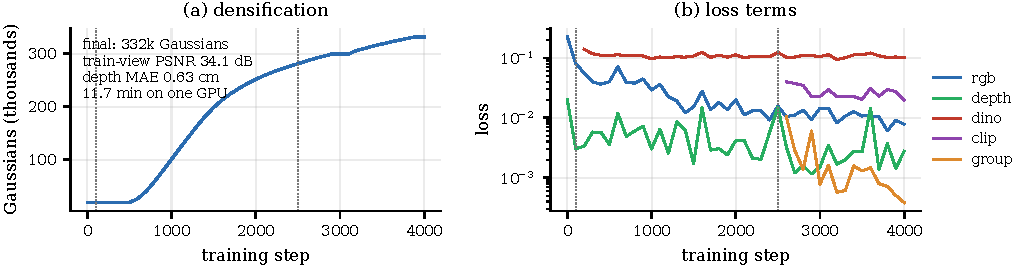
\includegraphics[width=\linewidth]{figures/training.pdf}
\caption{Training. (a) Number of Gaussians (densification); (b) loss terms on
a log scale. Dotted lines mark the start of DINO (step 100) and CLIP + grouping
supervision (step 2500).}
\label{fig:training}
\end{figure}

\begin{figure}[t]
\centering
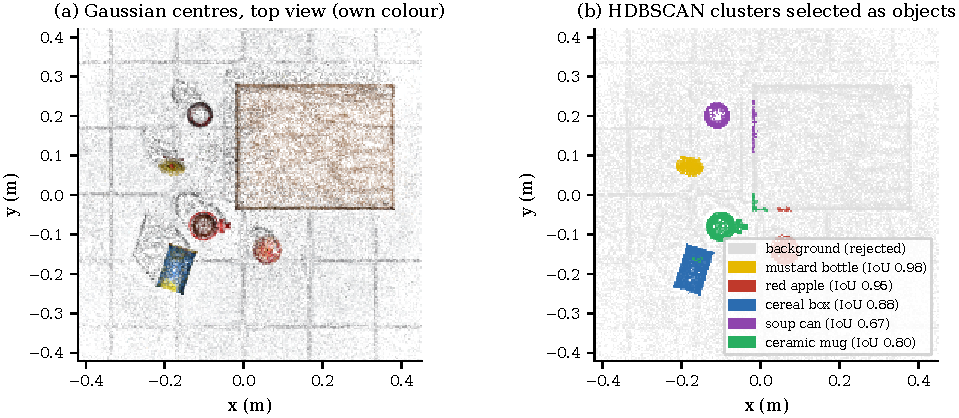
\includegraphics[width=\linewidth]{figures/grouping.pdf}
\caption{Grouping, top view of the Gaussian centres. (a) Each Gaussian in its
own colour. (b) The five clusters selected as objects; floor and table are
rejected. The IoU against the true Gaussians of each object is in the legend.}
\label{fig:grouping}
\end{figure}

\subsection{v1: base POGS per factor}

Figure~\ref{fig:factors} and Table~\ref{tab:factors-res} give the per-factor
results at the published budget of 25 iterations per frame. On the base case,
\pogs{} tracks the mug on 100\% of frames, with a median error of 0.78\,cm. The
benchmark separates the conditions clearly:
\begin{itemize}
  \item \textbf{Speed} is the sharpest limit: 100\% at 1$\times$, 82\% $\pm$ 31 at
        2$\times$ (one seed lost), and 40\% at 4$\times$, with 60\% of frames lost.
        Static gets 20\%.
  \item \textbf{Large rotations} degrade tracking with high seed variance: yaw 90
        reaches 49\%, tilt 30--60 and yaw+tilt 45 reach 59--66\%.
  \item \textbf{A hand occluding the object} breaks tracking: 43\% (partial) and
        34\% (heavy), with $\sim$53\% of frames lost. The gripper alone does not.
  \item \textbf{The cereal box} fails at 57\% $\pm$ 13: once the estimate lags,
        the rendered box overlaps floor pixels, and the depth term pulls it into
        the background (Fig.~\ref{fig:cases}).
  \item \textbf{Not discriminative} here: depth noise up to 10\,mm + 5\% holes
        (the 26\,cm ignore threshold absorbs it), the mustard bottle, and two
        objects moving at once. All are at $\approx$100\%.
\end{itemize}

\begin{figure}[t]
\centering
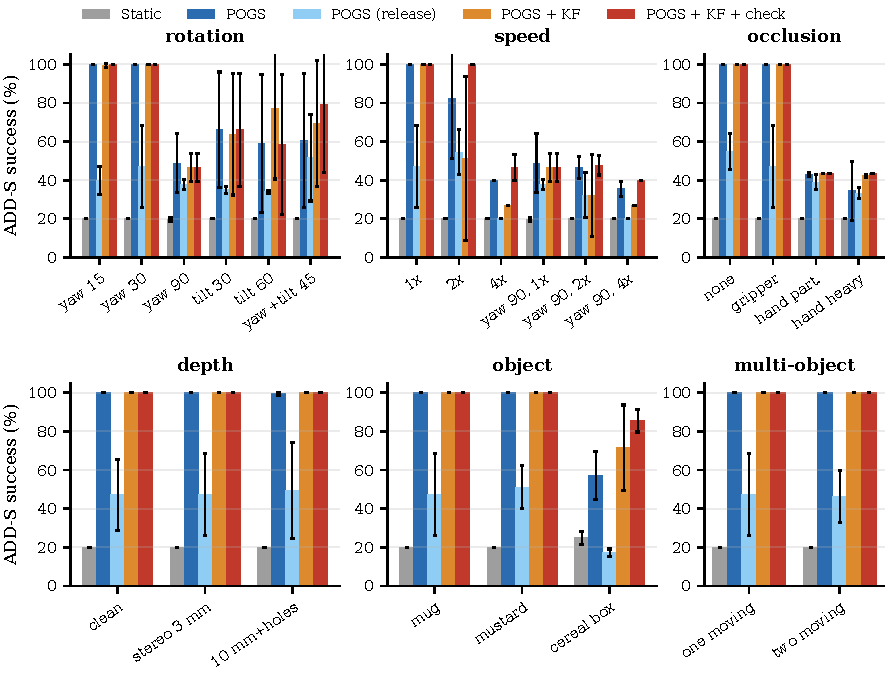
\includegraphics[width=\linewidth]{figures/factors.pdf}
\caption{ADD-S success per factor level (25 iterations per frame; mean over three
seeds, error bars = seed std). Static is the no-tracking floor.}
\label{fig:factors}
\end{figure}

\begin{table}[t]
\centering\footnotesize
\caption{Per-factor results at 25 iterations: ADD-S success $\pm$ seed std / lost-frame rate.
Best tracker per row in bold where methods differ.}
\label{tab:factors-res}
\setlength{\tabcolsep}{4pt}
\begin{tabular}{llccccc}
\toprule
Factor & Level & Static & POGS & POGS (release) & POGS + KF & POGS + KF + check \\
\midrule
\multirow{6}{*}{rotation}
 & yaw 15      & 20 / 73 & 100$\pm$0 / 0 & 40$\pm$7 / 11 & 99$\pm$1 / 0 & 100$\pm$0 / 0 \\
 & yaw 30      & 20 / 75 & 100$\pm$0 / 0 & 47$\pm$21 / 23 & 100$\pm$0 / 0 & 100$\pm$0 / 0 \\
 & yaw 90      & 19 / 75 & \best{49$\pm$15} / 21 & 38$\pm$3 / 43 & 47$\pm$7 / \best{10} & 47$\pm$7 / \best{10} \\
 & tilt 30     & 20 / 74 & \best{66$\pm$30} / 6 & 35$\pm$2 / 42 & 64$\pm$32 / 6 & \best{66$\pm$29} / 7 \\
 & tilt 60     & 20 / 67 & 59$\pm$36 / 37 & 34$\pm$1 / 39 & \best{77$\pm$37} / \best{18} & 58$\pm$36 / 22 \\
 & yaw+tilt 45 & 20 / 73 & 61$\pm$35 / 23 & 52$\pm$22 / 36 & 69$\pm$33 / \best{6} & \best{79$\pm$36} / 7 \\
\midrule
\multirow{6}{*}{speed}
 & 1$\times$   & 20 / 75 & 100$\pm$0 / 0 & 47$\pm$21 / 23 & 100$\pm$0 / 0 & 100$\pm$0 / 0 \\
 & 2$\times$   & 20 / 73 & 82$\pm$31 / 17 & 54$\pm$12 / 16 & 51$\pm$42 / 4 & \best{100$\pm$0} / \best{0} \\
 & 4$\times$   & 20 / 73 & 40$\pm$0 / 60 & 20$\pm$0 / 56 & 27$\pm$0 / 62 & \best{47$\pm$7} / \best{36} \\
 & yaw 90, 1$\times$ & 19 / 75 & \best{49$\pm$15} / 21 & 38$\pm$3 / 43 & 47$\pm$7 / \best{10} & 47$\pm$7 / \best{10} \\
 & yaw 90, 2$\times$ & 20 / 74 & 47$\pm$6 / 37 & 32$\pm$12 / 51 & 32$\pm$21 / \best{19} & \best{48$\pm$5} / 46 \\
 & yaw 90, 4$\times$ & 20 / 71 & 36$\pm$4 / 60 & 20$\pm$0 / 56 & 27$\pm$0 / 62 & \best{40$\pm$0} / \best{53} \\
\midrule
\multirow{4}{*}{occlusion}
 & none            & 20 / 76 & 100$\pm$0 / 0 & 55$\pm$9 / 0 & 100$\pm$0 / 0 & 100$\pm$0 / 0 \\
 & gripper         & 20 / 75 & 100$\pm$0 / 0 & 47$\pm$21 / 23 & 100$\pm$0 / 0 & 100$\pm$0 / 0 \\
 & + hand, partial & 20 / 76 & 43$\pm$1 / 54 & 39$\pm$4 / 54 & 43$\pm$0 / 54 & 43$\pm$0 / 54 \\
 & + hand, heavy   & 20 / 70 & 34$\pm$15 / 52 & 33$\pm$3 / 54 & 42$\pm$1 / 55 & \best{43$\pm$0} / 53 \\
\midrule
\multirow{3}{*}{depth}
 & clean           & 20 / 75 & 100$\pm$0 / 0 & 47$\pm$18 / 33 & 100$\pm$0 / 0 & 100$\pm$0 / 0 \\
 & stereo 3\,mm    & 20 / 75 & 100$\pm$0 / 0 & 47$\pm$21 / 23 & 100$\pm$0 / 0 & 100$\pm$0 / 0 \\
 & 10\,mm + holes  & 20 / 75 & 99$\pm$1 / 0 & 49$\pm$25 / 34 & 100$\pm$0 / 0 & 100$\pm$0 / 0 \\
\midrule
\multirow{3}{*}{object}
 & mug             & 20 / 75 & 100$\pm$0 / 0 & 47$\pm$21 / 23 & 100$\pm$0 / 0 & 100$\pm$0 / 0 \\
 & mustard bottle  & 20 / 73 & 100$\pm$0 / 0 & 51$\pm$11 / 5 & 100$\pm$0 / 0 & 100$\pm$0 / 0 \\
 & cereal box      & 25 / 70 & 57$\pm$13 / 31 & 17$\pm$2 / 59 & 72$\pm$22 / 14 & \best{86$\pm$6} / \best{0} \\
\midrule
\multirow{2}{*}{multi-object}
 & one moving      & 20 / 75 & 100$\pm$0 / 0 & 47$\pm$21 / 23 & 100$\pm$0 / 0 & 100$\pm$0 / 0 \\
 & two moving      & 20 / 69 & 100$\pm$0 / 0 & 46$\pm$13 / 33 & 100$\pm$0 / 0 & 100$\pm$0 / 0 \\
\bottomrule
\end{tabular}
\end{table}

\subsection{Paper ablations}

Table~\ref{tab:ablation} shows that per-frame depth is essential. Without it
(No Depth, and the release's depth-only-at-initialisation variant), success
drops to 44--47\% and the median error rises from 0.78\,cm to more than 6\,cm.
DINO matters less than in the paper: plain RGB also reaches 100\%, with a
slightly higher median error (1.09 vs.\ 0.78\,cm). The synthetic materials are
textured but simpler than real objects. On scene v1, which had flatter colours,
the two were indistinguishable.

\begin{table}[h]
\centering\small
\caption{Paper ablations on the base condition (3 seeds, 25 iterations).}
\label{tab:ablation}
\begin{tabular}{lcccc}
\toprule
Method & ADD-S success & Lost & Median pos.\ (cm) & Rot.\ err.\ (deg) \\
\midrule
Static (no motion)                       & 20\% & 75\% & 21.99 & 15.0 \\
POGS (DINO + depth every frame)          & \best{100\%} & \best{0\%} & \best{0.78} & 23.1 \\
No DINO (RGB + depth)                    & \best{100\%} & \best{0\%} & 1.09 & 22.7 \\
No Depth (DINO only)                     & 44\% & 17\% & 6.46 & 25.4 \\
POGS (release: depth only at init)       & 47\% & 23\% & 6.14 & 26.7 \\
\bottomrule
\end{tabular}
\end{table}

\subsection{Gripper-induced rotation error}
\label{sec:rot}

The rotation error is $\sim$23$^\circ$ even when position tracking is perfect.
Figure~\ref{fig:rotation} shows the cause. Without an occluder, the mug's
rotation error stays near 9$^\circ$, mostly yaw lag: the mug is nearly a cylinder,
and only the handle constrains yaw. With the gripper, the error rises to
$\sim$25$^\circ$ while the mug is held and recovers after release. The
gripper's depth lies in front of the mug, within the 26\,cm ignore threshold,
and the depth term tilts the estimate towards it. This is the occlusion
limitation of the paper in a mild form. It also explains why the
3\,cm\,\&\,5$^\circ$ rule saturates for every method.

\begin{figure}[h]
\centering
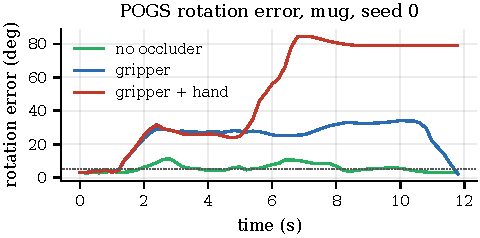
\includegraphics[width=0.55\linewidth]{figures/rotation.pdf}
\caption{\pogs{} rotation error on the mug (seed 0) without an occluder, with the
gripper, and with gripper + hand. The dotted line marks the paper's 5$^\circ$ threshold.}
\label{fig:rotation}
\end{figure}

\subsection{v2: Kalman motion prior}

\paragraph{Per factor.} At 25 iterations (Table~\ref{tab:factors-res}), the
loss-checked filter is never meaningfully worse than \pogs{} on success, and it
clearly helps in three places:
\begin{itemize}
  \item 2$\times$ speed: 100\% on every seed, against 82\% $\pm$ 31.
  \item 4$\times$ speed: 47\% with 36\% lost, against 40\% with 60\% lost.
  \item The cereal box: 86\% $\pm$ 6 with no lost frames, against 57\% $\pm$ 13
        with 31\% lost.
\end{itemize}
On large rotations, the KF variants roughly halve the lost-frame rate (yaw 90:
10\% vs.\ 21\%; yaw+tilt 45: 7\% vs.\ 23\%), but success changes within the seed
spread. Hand occlusion is unchanged: no variant reaches the object while it is
hidden. The plain KF without the check is unreliable. At 2$\times$ it reaches
51\% $\pm$ 42 (one seed perfect, the others lost), and it is worse than \pogs{}
on several levels.

\paragraph{Compute budget.} Figure~\ref{fig:budget} and Table~\ref{tab:budget}
summarise all 54 cases. At 25 and at 10 iterations, the loss-checked filter has
the highest success and the lowest lost rate. The extra loss evaluation costs
6--20\% more time per frame. At 10
iterations (3.6\,Hz) it matches \pogs{} at 25 iterations (70\% vs.\ 71\%) at
twice the frame rate, though it loses more frames (24\% vs.\ 22\%). At 5
iterations the prior hurts: plain KF collapses to 31\%, and even with the check
it reaches only 44\%, below \pogs{} at 5 iterations (55\%). A weak optimiser
cannot correct a wrong warm start, and the error feeds back into the velocity.
The KF variants also have higher mean rotation error (34--52$^\circ$ vs.\ 28--36$^\circ$),
because the prior extrapolates any spurious angular velocity.

\begin{figure}[t]
\centering
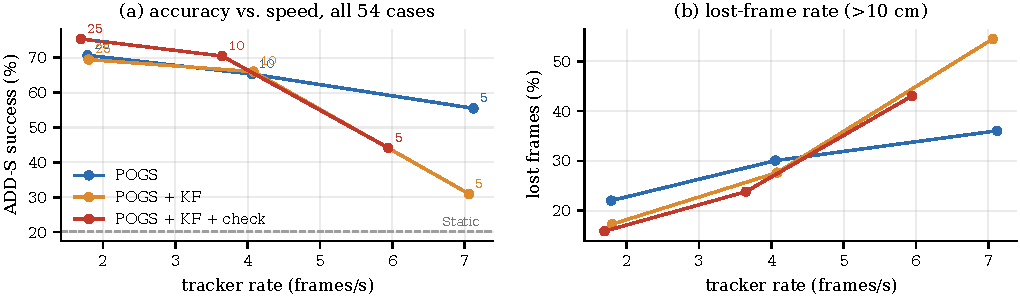
\includegraphics[width=\linewidth]{figures/budget.pdf}
\caption{Accuracy vs.\ tracker rate over all 54 offline cases. Labels give the
optimiser iterations per frame. (a) ADD-S success; (b) lost-frame rate.}
\label{fig:budget}
\end{figure}

\begin{table}[t]
\centering\small
\caption{Compute budget, all 54 offline cases (rate = mean frames per second
during tracking on an RTX 4070).}
\label{tab:budget}
\begin{tabular}{lccccccc}
\toprule
Method & Iters & Rate (Hz) & ADD-S success & Lost & Median pos.\ (cm) & Rot.\ err.\ (deg) \\
\midrule
POGS                         & 25 & 1.8 & 71\% & 22\% & 8.6 & 35.6 \\
POGS + KF                    & 25 & 1.8 & 69\% & 17\% & 9.9 & 41.7 \\
POGS + KF + check            & 25 & 1.7 & \best{75\%} & \best{16\%} & \best{6.4} & 40.1 \\
\midrule
POGS                         & 10 & 4.1 & 65\% & 30\% & 9.5 & 28.5 \\
POGS + KF                    & 10 & 4.1 & 66\% & 28\% & 11.4 & 41.1 \\
POGS + KF + check            & 10 & 3.6 & \best{70\%} & \best{24\%} & \best{9.4} & 33.9 \\
\midrule
POGS                         & 5  & 7.1 & \best{55\%} & \best{36\%} & \best{11.0} & 28.0 \\
POGS + KF                    & 5  & 7.1 & 31\% & 54\% & 29.4 & 51.6 \\
POGS + KF + check            & 5  & 5.9 & 44\% & 43\% & 15.5 & 38.1 \\
\bottomrule
\end{tabular}
\end{table}

\paragraph{Speed vs.\ budget.} Figure~\ref{fig:speed} crosses the speed factor
with the budget. The benefit of the prior grows with object speed only when the
optimiser has enough iterations to refine the warm start. At 25 iterations, the
check variant is flat at 100\% up to 2$\times$. At 10 iterations it still
improves 2$\times$ (66\% vs.\ 50\%). At 5 iterations it is worse than \pogs{}
even at 1$\times$.

\begin{figure}[t]
\centering
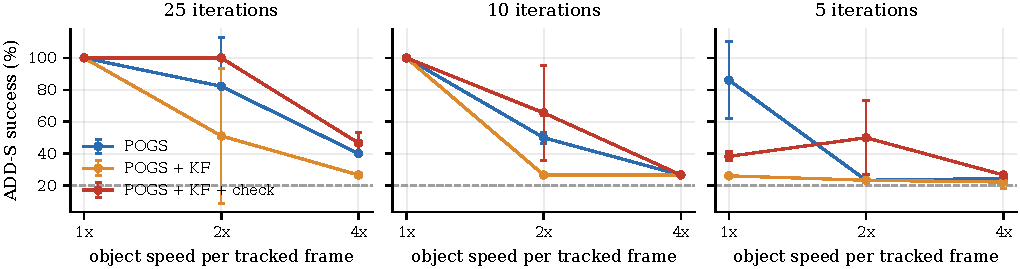
\includegraphics[width=\linewidth]{figures/speed.pdf}
\caption{ADD-S success vs.\ object speed per tracked frame (base trajectory, mean
$\pm$ seed std) at three optimiser budgets. Dashed: Static.}
\label{fig:speed}
\end{figure}

\paragraph{Case studies.} Figure~\ref{fig:cases} shows per-frame position errors
for four seed-0 cases.
\begin{itemize}
  \item 2$\times$ speed: \pogs{} falls behind during the carry and never
        recovers, while both KF variants stay below 2\,cm.
  \item Cereal box: \pogs{} and KF + check track it, but the plain KF diverges
        near placement.
  \item Tilt 60: the plain KF follows the object, while \pogs{} and KF + check
        lose it at peak tilt, when the unscanned underside faces the camera.
  \item Heavy hand occlusion: every method loses the mug when the hand covers
        it, and the plain KF then extrapolates it away at the speed limit.
\end{itemize}
These cases show why the plain KF is high-variance: the same mechanism that
rescues a lagging estimate also amplifies a wrong one.

\begin{figure}[t]
\centering
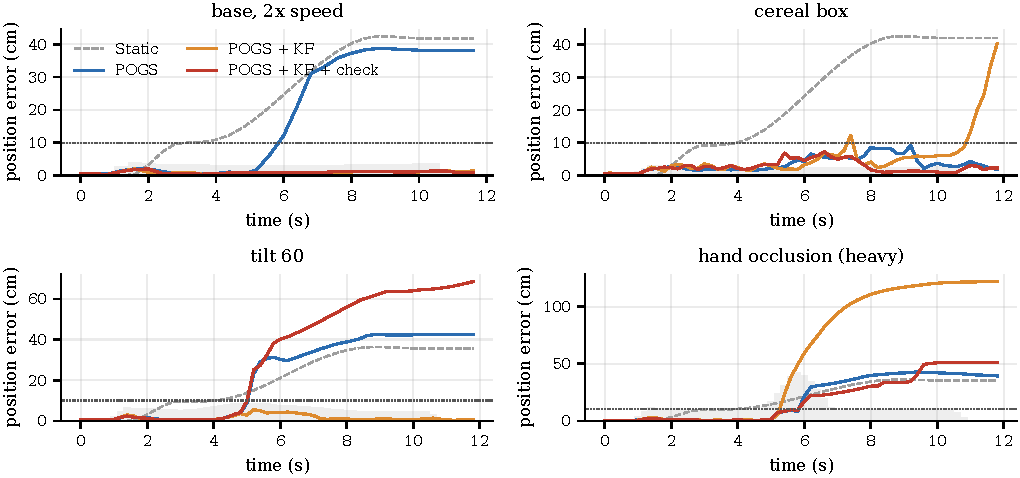
\includegraphics[width=\linewidth]{figures/cases.pdf}
\caption{Per-frame position error, seed 0. Grey shading shows how much of the
target is occluded; the dotted line marks the 10\,cm ``lost'' threshold.}
\label{fig:cases}
\end{figure}

\subsection{v3: other objects and two moving objects}

The mustard bottle is tracked at 100\% by every depth-using method, with a lower
rotation error than the mug (8$^\circ$ vs.\ 23$^\circ$): it is tall, and the
gripper hides less of it. The cereal box is the hardest object
(Table~\ref{tab:factors-res}). Its large flat faces sit close to the floor, so a
lagging estimate overlaps background depth. The loss check is what makes the KF
safe here: 86\% vs.\ 72\% for the plain KF. With two objects moving at once (mug
and soup can, each tracked with its own transform), all depth-using methods stay
at 100\%. The cost per frame roughly doubles (about 1.0\,s for \pogs{}), because
each object has its own ROI render. The KF variants have a lower median error
(0.60--0.70\,cm vs.\ 0.96\,cm).

\subsection{Real-time tracking}

Table~\ref{tab:rt} and Figures~\ref{fig:rt_bars}--\ref{fig:rt_error} give the
real-time results on the base trajectory at 1$\times$ and 2$\times$ playback.

\begin{table}[t]
\centering\small
\caption{Real-time results (30\,Hz camera, base trajectory, 3 seeds). ``Now''
scores the published pose at every camera frame. Latency is the measured compute
per tracked frame; age is the mean age of the camera frame behind the published
pose.}
\label{tab:rt}
\setlength{\tabcolsep}{4pt}
\begin{tabular}{lcccccccc}
\toprule
& & & \multicolumn{3}{c}{1$\times$ playback} & & \multicolumn{2}{c}{2$\times$ playback} \\
\cmidrule(lr){4-6}\cmidrule(lr){8-9}
Method & Latency & Rate & Success (now) & Lost & Median (cm) & Age & Success (now) & Lost \\
\midrule
Static (no motion)                & --     & --     & 19\% & 76\% & 21.99 & -- & 19\% & 76\% \\
POGS                              & 526\,ms & 1.9\,Hz & 56\%\,$\pm$\,19 & 19\% & 9.16 & 802\,ms & 20\% & 59\% \\
POGS, 10 iters                    & 225\,ms & 4.4\,Hz & \best{100\%}\,$\pm$\,1 & \best{0\%} & 1.69 & 354\,ms & 25\% & 48\% \\
POGS + KF + check                 & 540\,ms & 1.9\,Hz & 66\%\,$\pm$\,2 & 1\% & 2.89 & 824\,ms & 26\% & 42\% \\
\quad + latency comp.             & 540\,ms & 1.9\,Hz & 91\%\,$\pm$\,3 & \best{0\%} & 2.09 & 824\,ms & \best{34\%} & \best{29\%} \\
POGS + KF + check, 10 iters       & 253\,ms & 4.0\,Hz & 97\%\,$\pm$\,3 & \best{0\%} & 1.86 & 396\,ms & 20\% & 53\% \\
\quad + latency comp.             & 253\,ms & 4.0\,Hz & \best{100\%}\,$\pm$\,0 & \best{0\%} & \best{1.49} & 396\,ms & 23\% & 49\% \\
\bottomrule
\end{tabular}
\end{table}

\paragraph{Published POGS cannot keep up.} At 526\,ms per frame, \pogs{}
processes one of every $\sim$15 camera frames (Fig.~\ref{fig:rt_schedule}a). The
pose it publishes is on average 0.8\,s old and up to 1.2\,s old
(Fig.~\ref{fig:rt_schedule}b). The same trajectory that it tracks perfectly
offline now yields 56\% $\pm$ 19 success, and on one seed the mug is lost for
good (Fig.~\ref{fig:rt_error}, left). Speed is the main fix: \pogs{} at 10
iterations runs at 4.4\,Hz and is right on 100\% of frames.

\paragraph{Latency compensation.} Extrapolating the published estimate to the
current time (Eq.~\ref{eq:extrap}) is free at run time and helps most when the
tracker is slow. At 25 iterations it raises KF + check from 66\% to 91\%. At 10
iterations it reaches 100\% with the lowest median error of all methods
(1.49\,cm vs.\ 1.69\,cm for \pogs{} at 10 iterations). The saw-tooth error in
Fig.~\ref{fig:rt_error} (left) is the estimate ageing between updates;
compensation flattens it.

\paragraph{2$\times$ playback breaks everything.} With the stream played twice as
fast, every method falls to 20--34\%. The best is KF + check + latency
compensation at 25 iterations (34\% $\pm$ 17, 29\% lost), but with high variance
across seeds. The motion prior does not rescue the 10-iteration tracker here.

\begin{figure}[t]
\centering
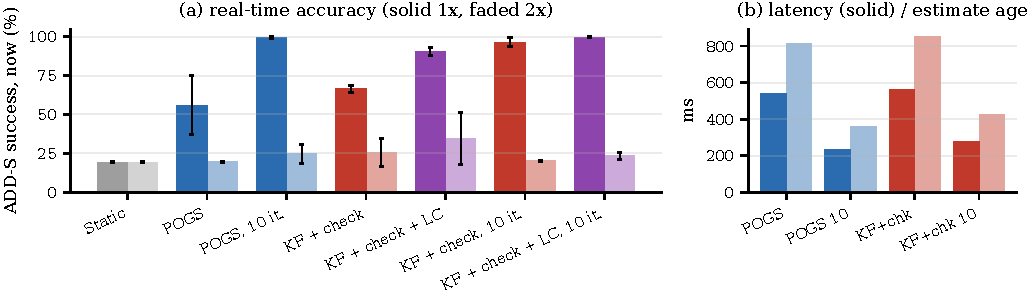
\includegraphics[width=\linewidth]{figures/rt_bars.pdf}
\caption{Real-time summary over three seeds. (a) ADD-S success scored at every
camera frame (solid 1$\times$, faded 2$\times$ playback). (b) Latency per
tracked frame (solid) and mean estimate age (faded).}
\label{fig:rt_bars}
\end{figure}

\begin{figure}[t]
\centering
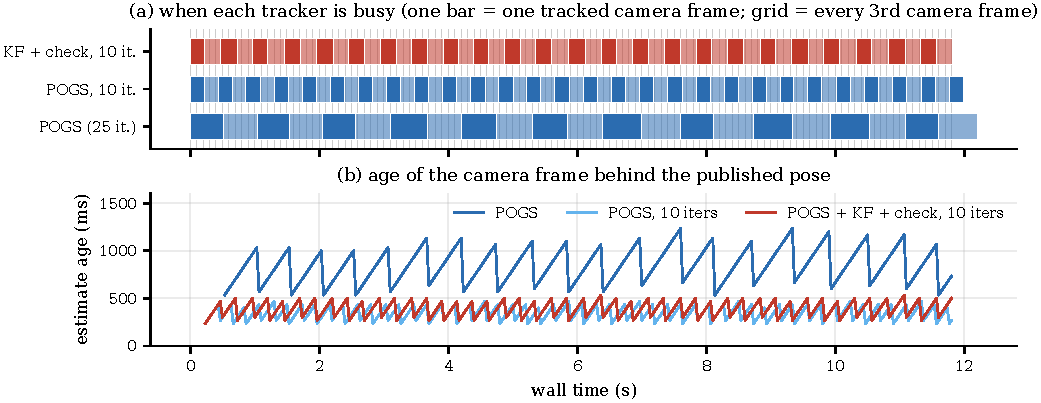
\includegraphics[width=\linewidth]{figures/rt_schedule.pdf}
\caption{Real-time schedule, base seed 0, 1$\times$. (a) Compute intervals: each bar
is one tracked camera frame; every other bar is lighter to show the boundaries.
(b) Age of the camera frame behind the published pose: it rises until the next
estimate is published, then drops.}
\label{fig:rt_schedule}
\end{figure}

\begin{figure}[t]
\centering
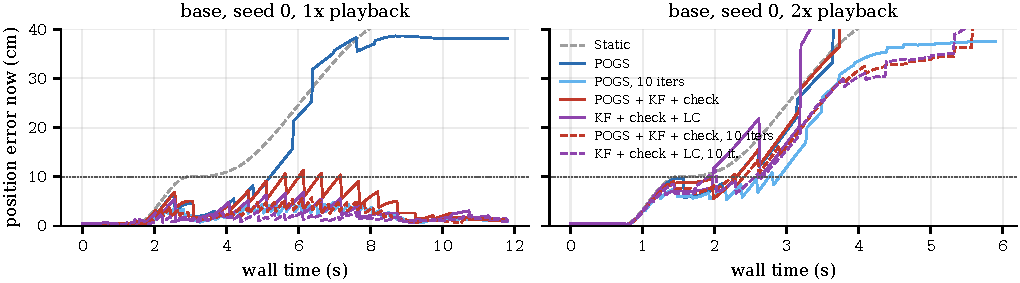
\includegraphics[width=\linewidth]{figures/rt_error.pdf}
\caption{Position error of the published pose at every camera frame, base seed 0.
LC = latency compensation. Dashed purple and red: the 10-iteration KF variants.}
\label{fig:rt_error}
\end{figure}

\paragraph{Visual output.} Every run can produce a dashboard video
(Fig.~\ref{fig:dash}). It shows the camera image with ground-truth (green) and
estimated (cyan) boxes, the object splats rendered at the estimate over the
image, the raw Gaussian scene with the tracked object moved to the estimate, and
the raw object splats alone. Live text gives the latency, the tracker rate, the
frame behind the shown estimate, its age, and the frames skipped.

\begin{figure}[p]
\centering
\begin{subfigure}{\linewidth}\centering
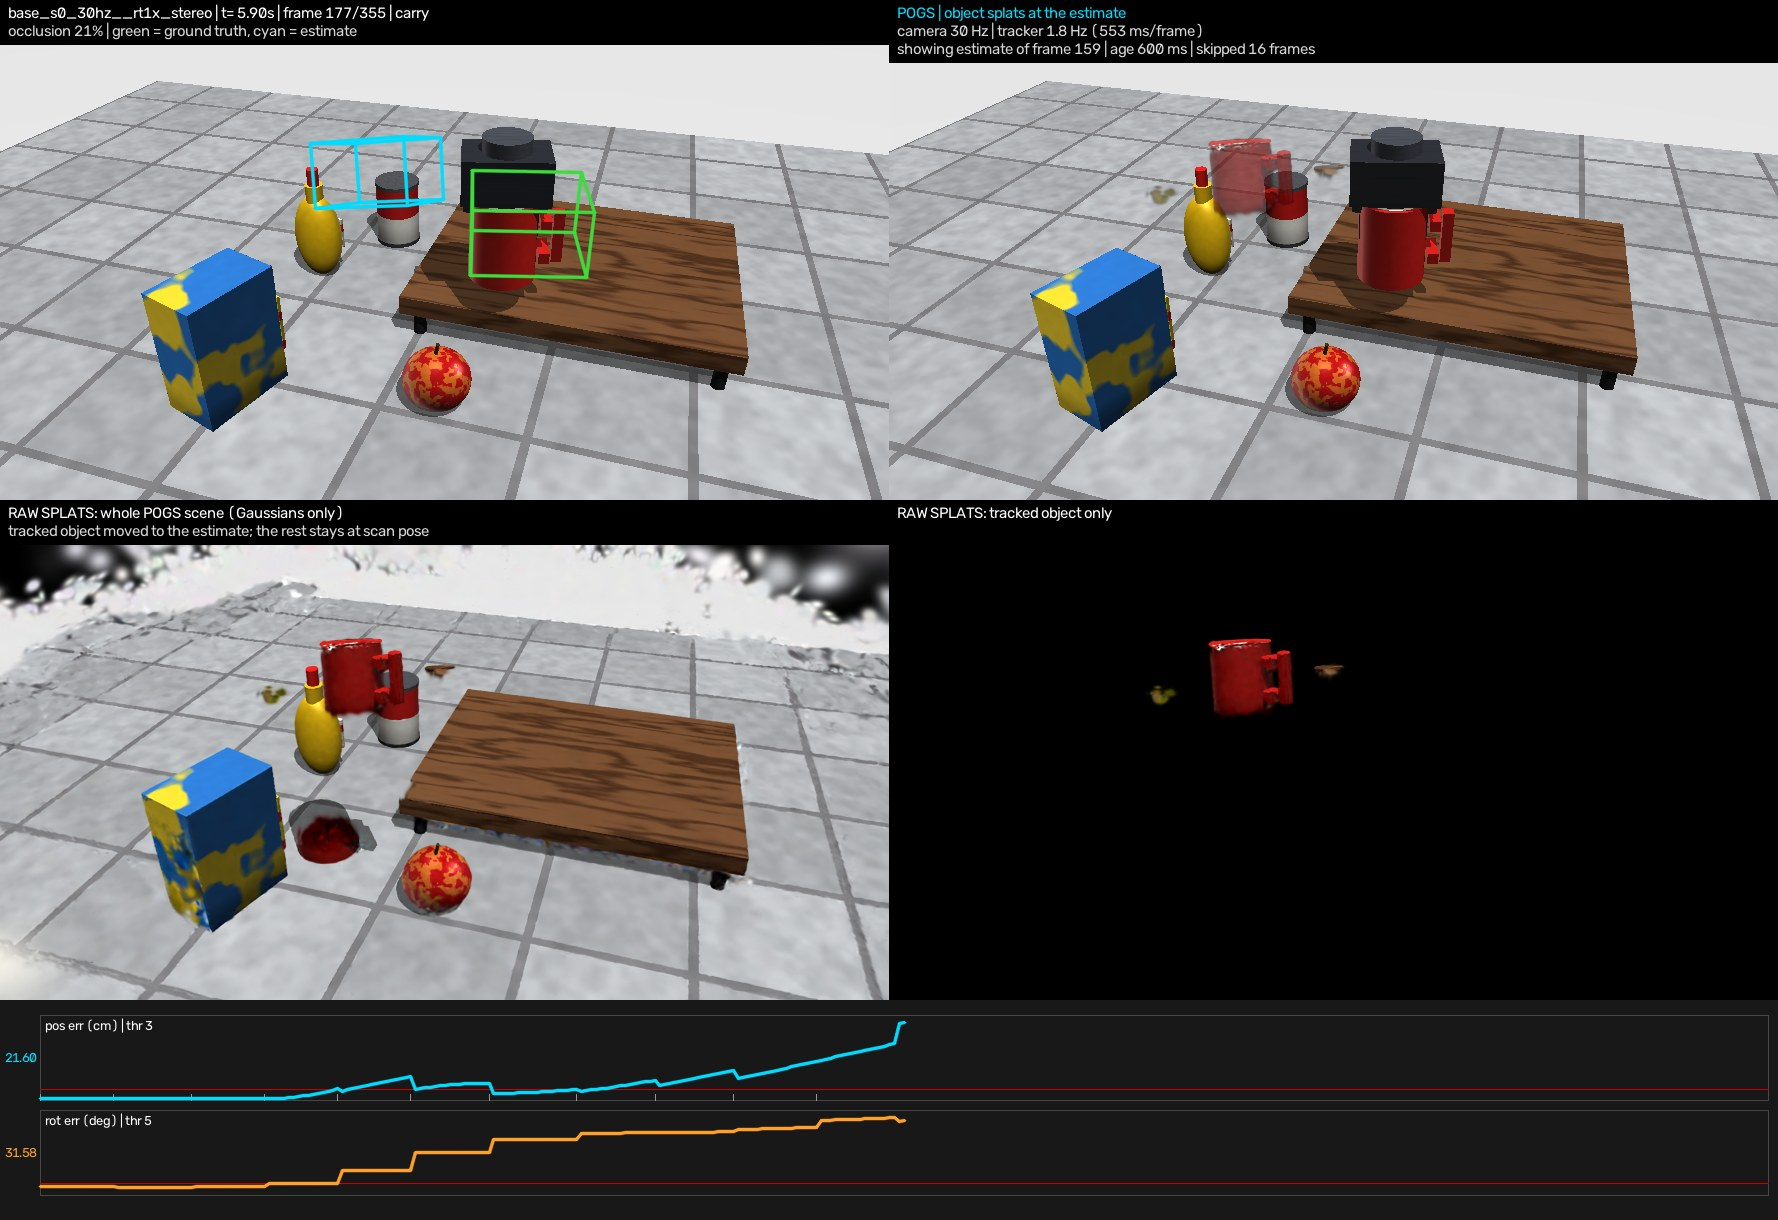
\includegraphics[width=0.92\linewidth]{figures/dash_rt_pogs.jpg}
\caption{\pogs{} (25 iterations, 1.8\,Hz): the shown estimate is 600\,ms old (16
frames skipped), and the object splats sit on the soup can while the mug is
already on the table.}
\end{subfigure}\\[0.6em]
\begin{subfigure}{\linewidth}\centering
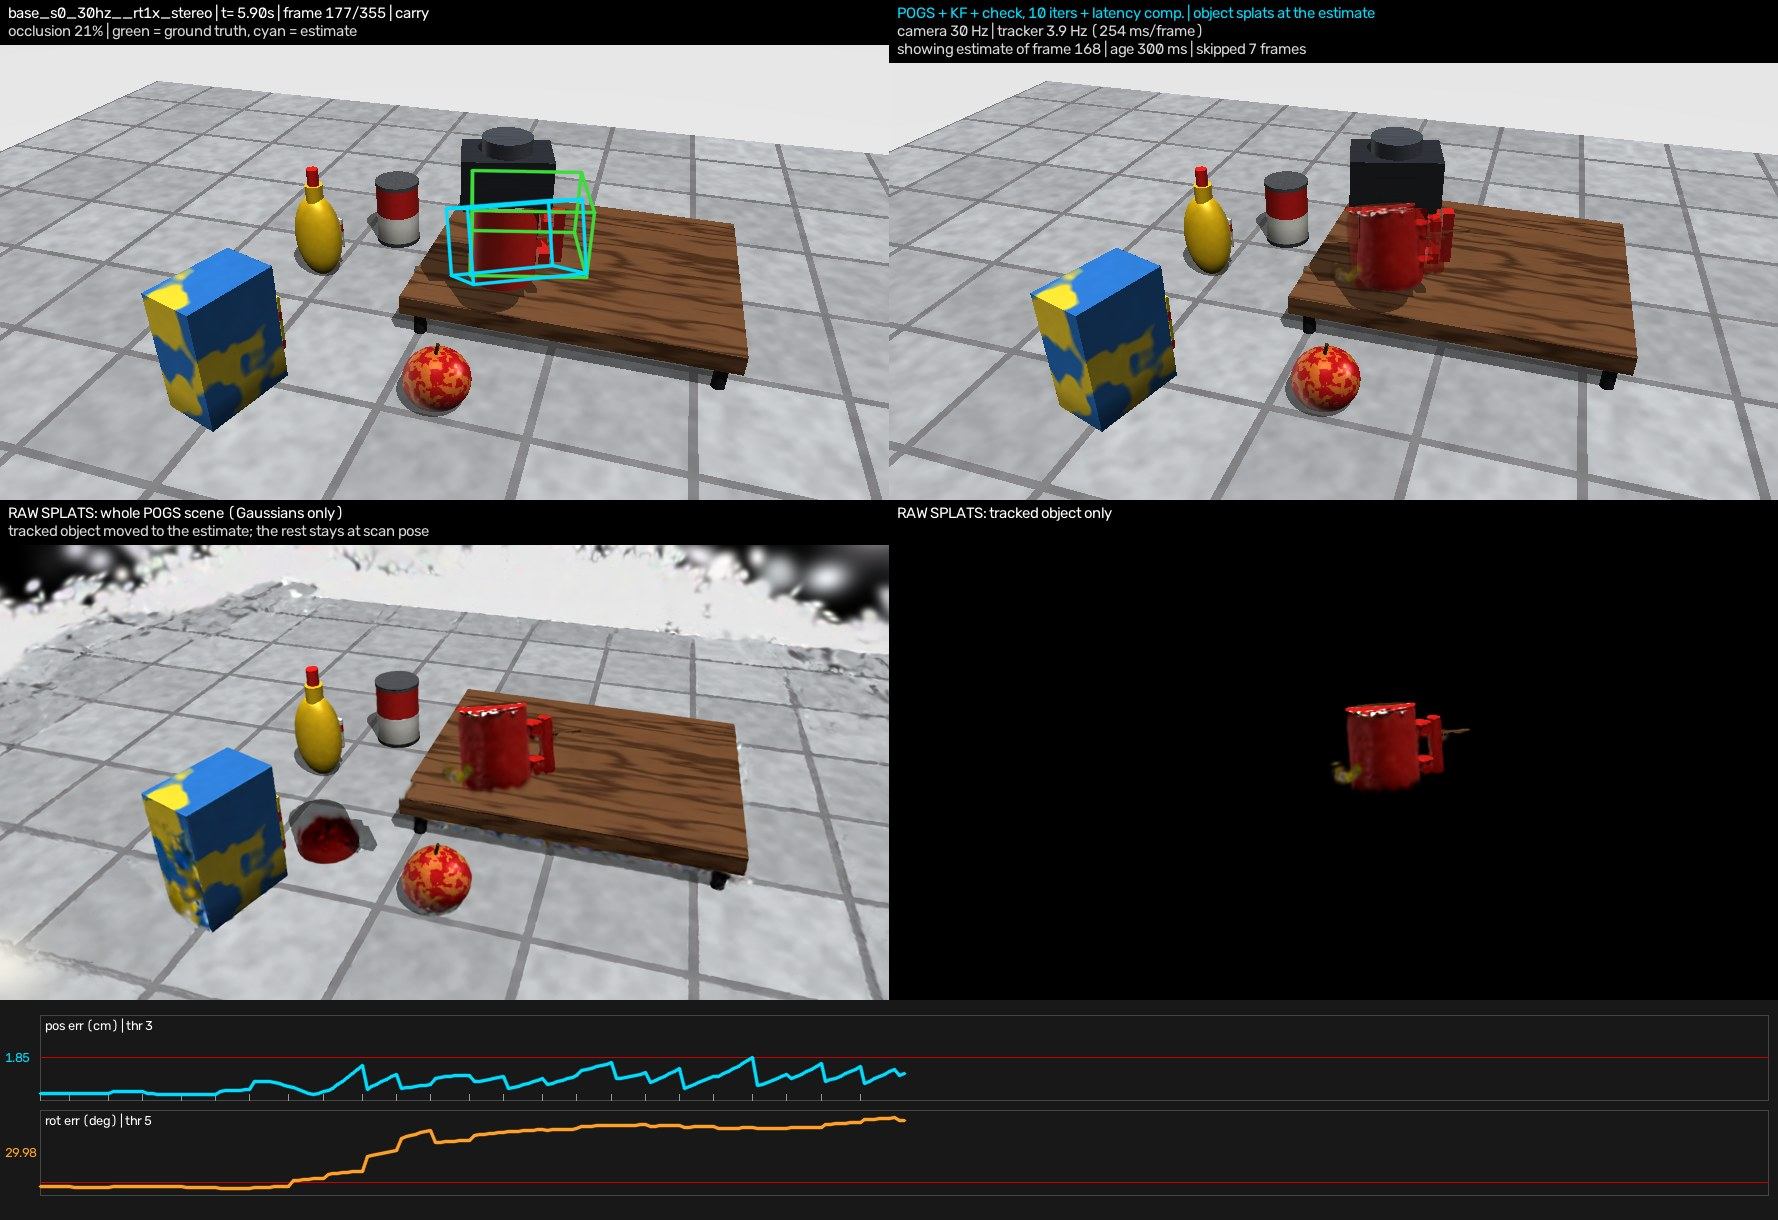
\includegraphics[width=0.92\linewidth]{figures/dash_rt_kf.jpg}
\caption{\pogs{} + KF + check, 10 iterations + latency compensation (3.9\,Hz): the
estimate is 300\,ms old and extrapolated to now; the splats follow the mug.}
\end{subfigure}
\caption{Real-time dashboards, base seed 0, frame 177 of 355 (mid-carry). The
panels show the camera image with boxes, the splat overlay, the raw full-scene
splats, and the raw object splats, above the error timeline.}
\label{fig:dash}
\end{figure}

%==========================================================================
\section{Discussion}
\label{sec:discussion}
%==========================================================================

\paragraph{What the benchmark shows about POGS.} On slow motion, \pogs{} is
accurate: sub-centimetre median error, robust to depth noise, two objects at
once, and a thin bottle. Its limits are those the paper names, and the benchmark
now quantifies them. Accuracy collapses once the per-frame motion exceeds what 25
Adam steps can follow (2--4$\times$). A hand covering the object loses it
outright. Large rotations that expose unscanned faces are unreliable, with high
seed variance. Compute time turns the speed limit into a real-time problem:
at 1.9\,Hz on a 30\,Hz stream, even normal-speed motion is tracked on only
about half of the frames.

\paragraph{What the Kalman prior does and does not do.} A warm start helps only
when the optimiser can verify and refine it. With the loss check and at least 10
iterations, it is the best method overall and solves the 2$\times$ and cereal-box
failures. Without the check, or with 5 iterations, it is unsafe. The optimiser's
output is not independent of the prediction, so a wrong prediction confirms
itself, and the filter carries a lost object away at the speed limit. Damping and
speed limits bound the damage but do not remove it. The real-time results put
the gains in proportion: making the tracker fast (10 iterations) is worth more
than the motion prior, and the cheapest single improvement is extrapolating the
published pose to the current time.

\paragraph{Limitations of this study.}
\begin{itemize}
  \item The data are synthetic: one scene, one trained model, rigid objects, a
        static camera, and an analytic renderer. Absolute numbers are not
        comparable with the paper's physical-robot results, which measured
        placement error with calipers (2.5--4.1\,cm, Table~I of~\cite{pogs}) and
        tool-servo success rates.
  \item Three seeds per level give large standard deviations on the hard levels;
        differences within one standard deviation should not be over-read.
  \item Grouping uses rendered instance masks and geometric selection instead of
        Detic and an operator's click.
  \item Real-time timings are for one RTX 4070 and include only tracking compute
        (DINO features + optimisation). Initialisation is untimed.
  \item Rotation error is dominated by the gripper-induced tilt, so the paper's
        3\,cm\,\&\,5$^\circ$ rule cannot rank methods here.
\end{itemize}

\paragraph{Next steps.} Occlusion is the clearest open problem: no variant
handles a hand over the object. Promising directions include
occlusion-aware depth residuals (masking the known gripper, or rejecting depth
in front of the rendered object), holding the motion prior's pose instead of
optimising while the object is mostly hidden, and gating Kalman updates by NIS.
For real time, the largest gains are likely from cheaper per-frame features and
asynchronous extrapolation at the camera rate.

%==========================================================================
\section{Conclusion}
%==========================================================================

We re-implemented \pogs{} from the paper and the authors' release, and built a
controlled synthetic benchmark around the limitations the paper reports. On it,
we evaluated a Kalman motion prior and a real-time protocol driven by measured
latency. \pogs{} is accurate on slow motion but fails at higher speeds, under
hand occlusion and on large rotations. As published, it is too slow for a live
30\,Hz camera: right on 56\% of frames, with poses 0.8\,s old. A loss-checked
SE(3) Kalman warm start is the most accurate method offline (75\% vs.\ 71\%
success; 100\% vs.\ 82\% at twice the speed; 86\% vs.\ 57\% on the cereal box).
Combined with fewer iterations and latency compensation, it tracks the
real-time stream on 100\% of frames with the lowest error. The prior is unsafe
without the loss check or with a very small iteration budget, and hand
occlusion remains unsolved.

\paragraph{Reproducibility.} All code, data generators, cached runs and videos
are in the repository. The full pipeline runs with
\begin{verbatim}
.venv/bin/python -m scene_generator.preview_scene       # optional scene preview (CPU)
.venv/bin/python -m experiments.v1_base_pogs.run_all    # data, train, group, track, videos
.venv/bin/python -m experiments.v2_kalman_pogs.run_all
.venv/bin/python -m experiments.v3_scene_mustard.run_all
.venv/bin/python -m experiments.realtime.run_all        # 30 Hz data + real-time protocol
.venv/bin/python -m experiments.results_tables          # tables (CPU)
.venv/bin/python report/make_figures.py                 # this report's figures (CPU)
\end{verbatim}
The full suite took about 4.3\,h of GPU time on one RTX 4070 (training 12\,min,
v1 69\,min, v2 2.8\,h, real time 12\,min).

\begin{thebibliography}{99}\small
\bibitem{pogs} J.~Yu, K.~Hari, K.~El-Refai, A.~Dalal, J.~Kerr, C.~M.~Kim, R.~Cheng,
  M.~Z.~Irshad, K.~Goldberg. Persistent Object Gaussian Splat (POGS) for Tracking
  Human and Robot Manipulation of Irregularly Shaped Objects. \emph{ICRA}, 2025.
\bibitem{kerbl3dgs} B.~Kerbl, G.~Kopanas, T.~Leimk\"uhler, G.~Drettakis. 3D Gaussian
  Splatting for Real-Time Radiance Field Rendering. \emph{ACM TOG (SIGGRAPH)}, 2023.
\bibitem{dinov2} M.~Oquab et al. DINOv2: Learning Robust Visual Features without
  Supervision. \emph{TMLR}, 2024.
\bibitem{clip} A.~Radford et al. Learning Transferable Visual Models From Natural
  Language Supervision. \emph{ICML}, 2021.
\bibitem{lerf} J.~Kerr, C.~M.~Kim, K.~Goldberg, A.~Kanazawa, M.~Tancik. LERF: Language
  Embedded Radiance Fields. \emph{ICCV}, 2023.
\bibitem{garfield} C.~M.~Kim, M.~Wu, J.~Kerr, K.~Goldberg, M.~Tancik, A.~Kanazawa.
  GARField: Group Anything with Radiance Fields. \emph{CVPR}, 2024.
\bibitem{rsrd} J.~Kerr, C.~M.~Kim, M.~Wu, B.~Yi, Q.~Wang, K.~Goldberg, A.~Kanazawa.
  Robot See Robot Do: Imitating Articulated Object Manipulation with Monocular 4D
  Reconstruction. \emph{CoRL}, 2024.
\bibitem{nerfstudio} M.~Tancik et al. Nerfstudio: A Modular Framework for Neural
  Radiance Field Development. \emph{SIGGRAPH}, 2023.
\bibitem{gsplat} V.~Ye et al. gsplat: An Open-Source Library for Gaussian Splatting.
  \emph{arXiv:2409.06765}, 2024.
\bibitem{detic} X.~Zhou, R.~Girdhar, A.~Joulin, P.~Kr\"ahenb\"uhl, I.~Misra. Detecting
  Twenty-thousand Classes using Image-level Supervision. \emph{ECCV}, 2022.
\bibitem{hdbscan} R.~J.~G.~B.~Campello, D.~Moulavi, J.~Sander. Density-Based Clustering
  Based on Hierarchical Density Estimates. \emph{PAKDD}, 2013.
\bibitem{barshalom} Y.~Bar-Shalom, X.~R.~Li, T.~Kirubarajan. \emph{Estimation with
  Applications to Tracking and Navigation}. Wiley, 2001.
\bibitem{posecnn} Y.~Xiang, T.~Schmidt, V.~Narayanan, D.~Fox. PoseCNN: A Convolutional
  Neural Network for 6D Object Pose Estimation in Cluttered Scenes. \emph{RSS}, 2018.
\end{thebibliography}

\appendix
\section{Full speed $\times$ budget table}

\begin{table}[h]
\centering\small
\caption{Speed factor at three budgets: ADD-S success $\pm$ seed std / lost.}
\begin{tabular}{lcccccc}
\toprule
Level & POGS & KF + check & POGS, 10 & KF + check, 10 & POGS, 5 & KF + check, 5 \\
\midrule
1$\times$         & 100$\pm$0 / 0 & 100$\pm$0 / 0 & 100$\pm$0 / 0 & 100$\pm$0 / 0 & 86$\pm$24 / 11 & 38$\pm$3 / 47 \\
2$\times$         & 82$\pm$31 / 17 & 100$\pm$0 / 0 & 50$\pm$3 / 43 & 66$\pm$30 / 30 & 23$\pm$0 / 56 & 50$\pm$23 / 31 \\
4$\times$         & 40$\pm$0 / 60 & 47$\pm$7 / 36 & 27$\pm$0 / 56 & 27$\pm$0 / 56 & 24$\pm$4 / 60 & 27$\pm$0 / 58 \\
yaw 90, 1$\times$ & 49$\pm$15 / 21 & 47$\pm$7 / 10 & 52$\pm$15 / 34 & 48$\pm$8 / 37 & 41$\pm$4 / 49 & 37$\pm$3 / 39 \\
yaw 90, 2$\times$ & 47$\pm$6 / 37 & 48$\pm$5 / 46 & 40$\pm$7 / 51 & 46$\pm$8 / 36 & 22$\pm$2 / 58 & 27$\pm$9 / 50 \\
yaw 90, 4$\times$ & 36$\pm$4 / 60 & 40$\pm$0 / 53 & 24$\pm$4 / 60 & 27$\pm$0 / 58 & 22$\pm$4 / 64 & 24$\pm$4 / 58 \\
\bottomrule
\end{tabular}
\end{table}

\section{Software and data layout}
\begin{itemize}
  \item \texttt{scene\_generator/}: ray-caster, materials, scene, benchmark
        conditions, trajectory planner, dataset writer, scene preview.
  \item \texttt{common/}: model, trainer, encoders (DINO, CLIP), grouping,
        tracking (RigidGroupOptimizer), Kalman filter, evaluation (offline and
        real-time), checkpoint.
  \item \texttt{experiments/}: v1, v2, v3 and real-time drivers; shared pipeline;
        dashboard videos; result tables.
  \item \texttt{data\_results/}: per-experiment summaries, videos, and the shared
        run cache (\texttt{benchmark\_runs/\allowbreak<case>/\allowbreak<method>/}: row, telemetry, poses,
        real-time schedule).
  \item \texttt{report/}: this document and \texttt{make\_figures.py}.
\end{itemize}

\end{document}
